\section{Introduction}

In recent years, location privacy has become an increasingly concerned issue, and the preserving mechanisms based on differential privacy has proved to be the best way to resist background knowledge attacks. In the location privacy-preserving model based on differential privacy, there are two main implementation methods. One is based on the obfuscation on the number: constructing a spatial grid structure and adding noise to the number of workers in the grid; Another way is based on geo-obfuscation: obfuscating the real location of the worker and uploading it.

We mainly consider the geo-obfuscation in this paper. Miguel E. Andrés et al. proposed a location difference privacy framework based on Laplace obfuscation. In recent years, some scholars have put forward the implementation method of constructing linear programming model based on discrete obfuscation and demonstrated that this method could play a useful role in optimizing the travel distance and improving the coverage of target location.
Based on location privacy-preserving, we consider an essential performance evaluation index in crowdsourcing problems, which is the task acceptance rate. When the tasks are assigned to workers on a crowdsourcing platform, it is uncertain whether workers will accept the tasks. Rejection may occur with long travel distance or low reward, which is what crowdsourcing platform is trying to avoid when optimizing the allocation scheme. Therefore, we choose the worker's acceptance rate as the performance index. At the same time, we optimize and compare the task allocation mechanisms with mainstream privacy-preserving methods based on the location differential privacy model.

Moreover, not only performance but also overhead need to be considered in crowdsourcing problems. At the crowdsourcing server, bandwidth overhead and time overhead need to be considered. Since the crowdsourcing server needs to return all tasks within the area of retrieval (AOR) to the worker, the bandwidth overhead can be represented as area $S_{AOR}$. On the other hand, the time overhead depends on the different optimization methods. Comparing with the Laplace method, the method based on Benders Decomposition that allows the obfuscation function and task allocation strategy to iterate with each other requires more calculation overhead and correspondingly more time overhead. We will analyze the bandwidth overhead and time overhead respectively.
The main work of this paper is as follows:

1) Based on the framework of differential geo-obfuscation privacy-preserving, we introduce an improved model of the task acceptance rate in crowdsourcing problems. We also consider the task acceptance rate as the optimization goal from the perspective of task allocation.

2) We optimize the task acceptance rate and get the optimal solution using the current two mainstream obfuscation mechanisms under the framework of differential geo-obfuscation privacy-preserving. Considering the overhead of crowdsourcing server, we analyze and compare two obfuscation mechanisms from the perspective of bandwidth overhead and runtime overhead respectively.

3) By constructing a comprehensive evaluation model, we consider the tradeoff between privacy and bandwidth overhead and solve the optimal privacy budget choice.

\section{BACKGROUND}

\subsection{Spatial Crowdsourcing}
Crowdsourcing is aimed at ordinary users that have not explicitly been assigned, and they can all accept and complete published tasks on the platform. Spatial Crowdsourcing is a kind of crowdsourcing based on spatial geographic location. Its task is to assign a set of spatial tasks to workers so that workers can perform corresponding tasks at a specific workplace. As an online platform, spatial crowdsourcing currently has two main modes, one is the server assigned tasks (SAT), and the other is worker selected tasks (WST). For SAT mode, online workers on the platform need to send their location coordinates to the crowdsourcing server, which then assigns appropriate tasks to nearby workers. For WST mode, it requires requesters to publish online tasks on crowdsourcing platforms so that registered workers can independently select their nearby tasks based on the travel distance, and then the results are fed back to the platform, and communications with task requesters are established to complete the corresponding tasks. Up to now, SAT mode is still the current mainstream mode due to the consideration of assignment success rate (ASR).

\subsection{Differential Privacy}
\begin{definition}
	Differential privacy is defined on adjacent datasets. For two adjacent datasets $D_1$ and $D_2$, $Q$ is a randomized algorithm performing a query operation on the database. Let $Range(Q)$ denote the set of all possible outputs of the algorithm $Q$. We say that $Q$ satisfies the $\varepsilon$-differential-privacy mechanism if and only if the following inequality holds, $\forall S \in Range(Q)$:
	$$
	P_r[Q(D_1)=S]\leq e^\varepsilon \cdot P_r [Q(D_2)=S]
	$$
\end{definition}

Andrés et al. (2013) gave a basic framework of location privacy-preserving based on differential privacy mechanism and extended the concept of one-dimensional differential privacy to the two-dimensional plane. The key insight is that for any point $L_0 \in \mathbb R^2$ in the plane, an obfuscated point $L^* \in \mathbb R^2$ is generated near $L_0$ through a specific noise function. From the perspective of privacy-preserving of the user's location, the user uploads the obfuscated location $L^*$ instead of the real location $L_0$.

\begin{definition}
	The mechanism $M$ that takes a location as input satisfies $\varepsilon$-location-differential-privacy if the following inequality holds $\forall S \in Range(M)$: 
	$$
	\frac{P(S|L_1)}{P(S|L_2)} \leq e^{\varepsilon d(L_1,L_2)}
	$$
	$L_1$ and $L_2$ are two locations. $d(L_1,L_2)$ denotes the distance between the two locations. $\varepsilon$ denotes the privacy budget. 
\end{definition}
 The smaller $\varepsilon$ is, the closer the distributions of the two conditional probabilities are, which means that it is difficult for attackers to distinguish $L_1$ from $L_2$ based on the output $S$, hence the privacy is secured.

\section{FRAMEWORK}
\subsection{System Model}
The flowchart~\ref{img:SysModel} indicates the procedures of the geo-obfuscation in crowdsourcing model:

\begin{figure}
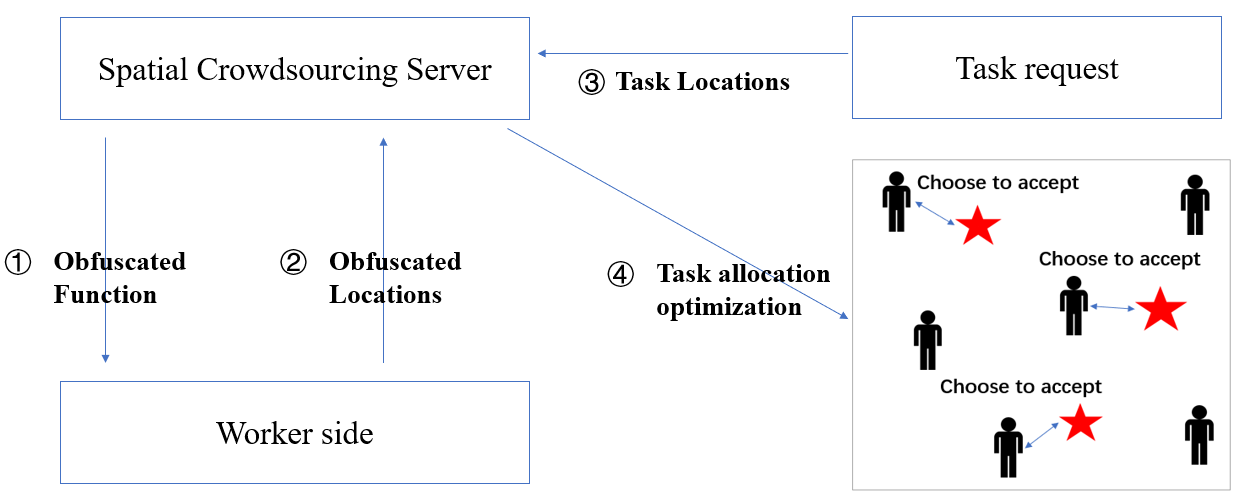
\includegraphics[width=8.5cm]{SysModel}
\label{img:SysModel}
\caption{System Model}
\end{figure}

The detailed procedures are as follow:
First, the crowdsourcing server generates the location obfuscation function based on the differential privacy framework and sends it to workers. After obfuscating the real location locally, the worker uploads the obfuscated location to the server. Meanwhile, the task requester uploads the location of the task to the server. The crowdsourcing server then optimizes the task allocation according to specific evaluation standards. Finally, the workers choose to accept or reject the tasks assigned to them.

Many of the current crowdsourcing platforms collect workers' location information directly, which can lead to the disclosure of workers' location privacy. However, by uploading the obfuscated location, the privacy of the location can be adequately protected. The privacy models will be analyzed in the next section.

Speaking of optimizing task allocation, Leye Wang (WWW' 17) optimized the planar crowdsourcing task allocation by minimizing the travel distance. However, in reality, workers accept the tasks assigned to them with a certain probability. If specific tasks assigned by the server are frequently rejected by workers, the overall performance of the platform will be significantly affected. Therefore, the overall task acceptance rate is the optimization goal in task allocation issue. The task acceptance rate will be modeled and analyzed later.

\subsection{Privacy Model}
The current mainstream privacy-preserving framework is based on the location differential privacy model. The location obfuscation function mentioned in the previous section also satisfies the definition of location differential privacy. Currently, there are two main generating mechanisms of obfuscation function, one is based on the Laplace mechanism, and the other is based on Benders Decomposition mechanism (Leye Wang, WWW'17).

\subsubsection{Planar Laplace Mechanism}
The most common mechanism in the field of location privacy-preserving uses planar Laplace distribution in the two-dimensional plane. Under planar Laplace obfuscation, the probability density of obfuscated point $L^*$ in the plane decreases exponentially as the distance from the real location $L_0$ increases. 

Given a privacy budget $\varepsilon$ and the real location $L_0 \in \mathbb R^2$, an obfuscated point $L^*$ can be obtained by adding noise on $L_0$. The probability density function of $L^*$ centered at $L_0$ is:
$$
	P_\varepsilon (L_0)(L^*)=\frac{\varepsilon^2}{2\pi} e^{-\varepsilon d(L_0,L^*)}
$$
$\frac{\varepsilon^2}{2\pi}$ is the normalization factor, and we call this function the planar Laplace function centered at $L_0$. It is obvious that the further away $L^*$ is from the center point $L_0$, the smaller the value of probability density is and decreasing exponentially.

\subsubsection{Benders Decomposition}
This method was first used to solve the linear programming problems. In this method, the location obfuscation function is discretized. In recent years, some scholars have proposed that the BD algorithm can be used to optimize the differential privacy problems. Unlike the Laplace mechanism described above, the location obfuscation function in this method is unknown, which means that two unknowns need to be solved for one optimization objective.

The basic idea of BD method is to use the definition of differential privacy to set up linear programming equations, and decompose the optimization problem into an obfuscation function problem (P-subproblem) and a task allocation problem (X-subproblem). The solution of each subproblem is substituted as a known parameter of the other subproblem so that each subproblem is transformed into a conventional linear programming problem that can be solved easily. Thus, the obfuscation mechanism and the task allocation mechanism can iterate over each other to find the optimal solution.

(Leye Wang WWW' 17) Wang used this method to optimize the travel distance of workers in crowdsourcing problems and decomposed the mixed integer nonlinear programming problem into two linear programming subproblems. Finally, Wang proved that this method could effectively reduce the overall travel distance of workers on the premise of satisfying the definition of differential privacy.

\subsection{Optimization Goal and Performance Analysis}
We introduced the task allocation process on the crowdsourcing platform earlier. Next, we consider the overall acceptance rate as the optimization goal of the actual situation. Moreover, system overhead is analyzed and compared, and further details emerge in a later section.

\subsubsection{Acceptance Rate}
When the crowdsourcing server assigns tasks to workers, workers need to further select appropriate tasks to complete. We use the acceptance rate ($AR$) to indicate the probability that workers will accept the task. A vital optimization goal in crowdsourcing is how to allocate tasks to workers reasonably to improve the overall task acceptance rate.

So far, most scholars in the crowdsourcing field used the univariate model to model $AR$. They believed that $AR$ is only related to the travel distance needed of workers, and expressed $AR$ as a function of travel distance. (Hien To, Differentially Private Location Protection for worker datasets in spatial crowdsourcing, IEEE Transactions on Mobile Computing16'). Two basic models are shown in graph~\ref{img:UniModel}:

\begin{figure}
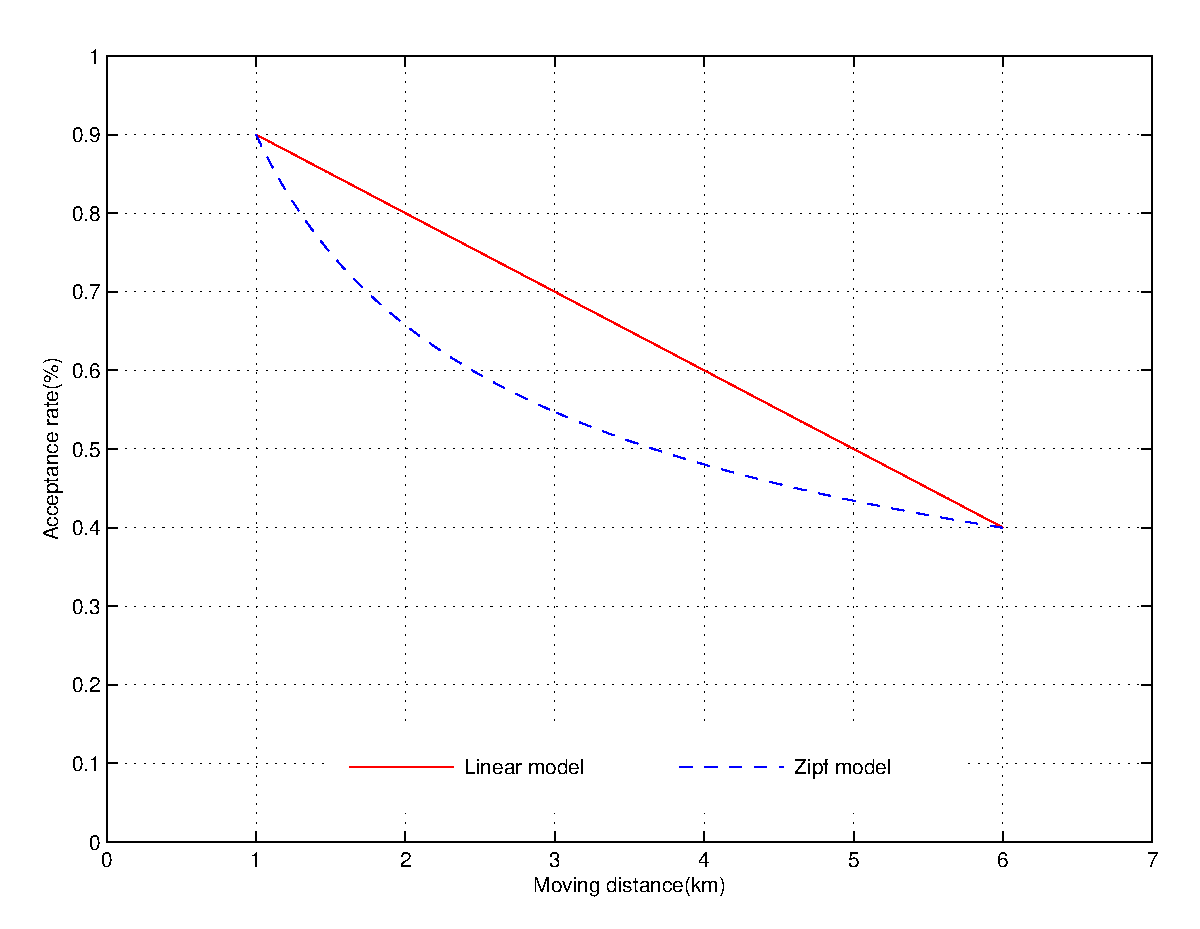
\includegraphics[width=8.5cm]{UniModel}
\label{img:UniModel}
\caption{Univariate Model of AR}
\end{figure}

Intuitively, this is one-sided. Therefore, we will introduce an improved bivariate model in a later section.

\subsubsection{System Overhead}
From the perspective of the crowdsourcing platform, tasks need to be assigned according to the locations uploaded by users, including searching for locations within the spatial area. On the other hand, crowdsourcing service based on LBS requires high real-time performance. As the scale of the problem, i.e., the number of workers ($N_w$) and the number of tasks ($N_t$), increases, the time spent on solving optimization problems will also increase accordingly. Therefore, it is necessary to analyze the overhead problem in the crowdsourcing model.

\section{ANALYSIS ON TASK ACCEPTANCE RATE IN CROWDSOURCING}
\subsection{Improvement of the Task Acceptance Rate Model}
In the analysis of task acceptance rate in crowdsourcing problems, previous papers only considered task acceptance rate as negatively correlated (linearly or exponentially) to travel distance. However, by considering the actual situation, whether workers accept tasks or not is affected not only by travel distance but also other factors. Therefore, we introduce the Reward factor for the tasks. In general, a higher reward for tasks is conducive to improving the probability which workers accept and complete tasks. We consider the linear model and hyperbolic tangent model respectively.

\subsubsection{Linear Model}
We firstly consider modeling the task acceptance rate with a linear model. Let $x_1=Rew/WTD$, where the $Rew$ denotes the reward of the task, $WTD$ denotes the travel distance of the worker. Within a certain range, $AR$ (acceptance rate) can be expressed as a linear function with respect to $x_1$. Considering the actual situation, when the reward is high enough, or the distance is close enough, the worker will hardly reject the task. $k_1$ is defined as the threshold, so when $x_1$ exceeds $k_1$, $AR$ is set to $1$.~\ref{img:LinTanh}
$$
	AR= \left \{
	\begin{array}{cl}
	\frac{x_1}{k_1} \quad & \mbox{$x_1<k_1$} \\
	1 \quad & \mbox{$x_1 \geq k_1$}
	\end{array}
	\right.
$$

\begin{figure}
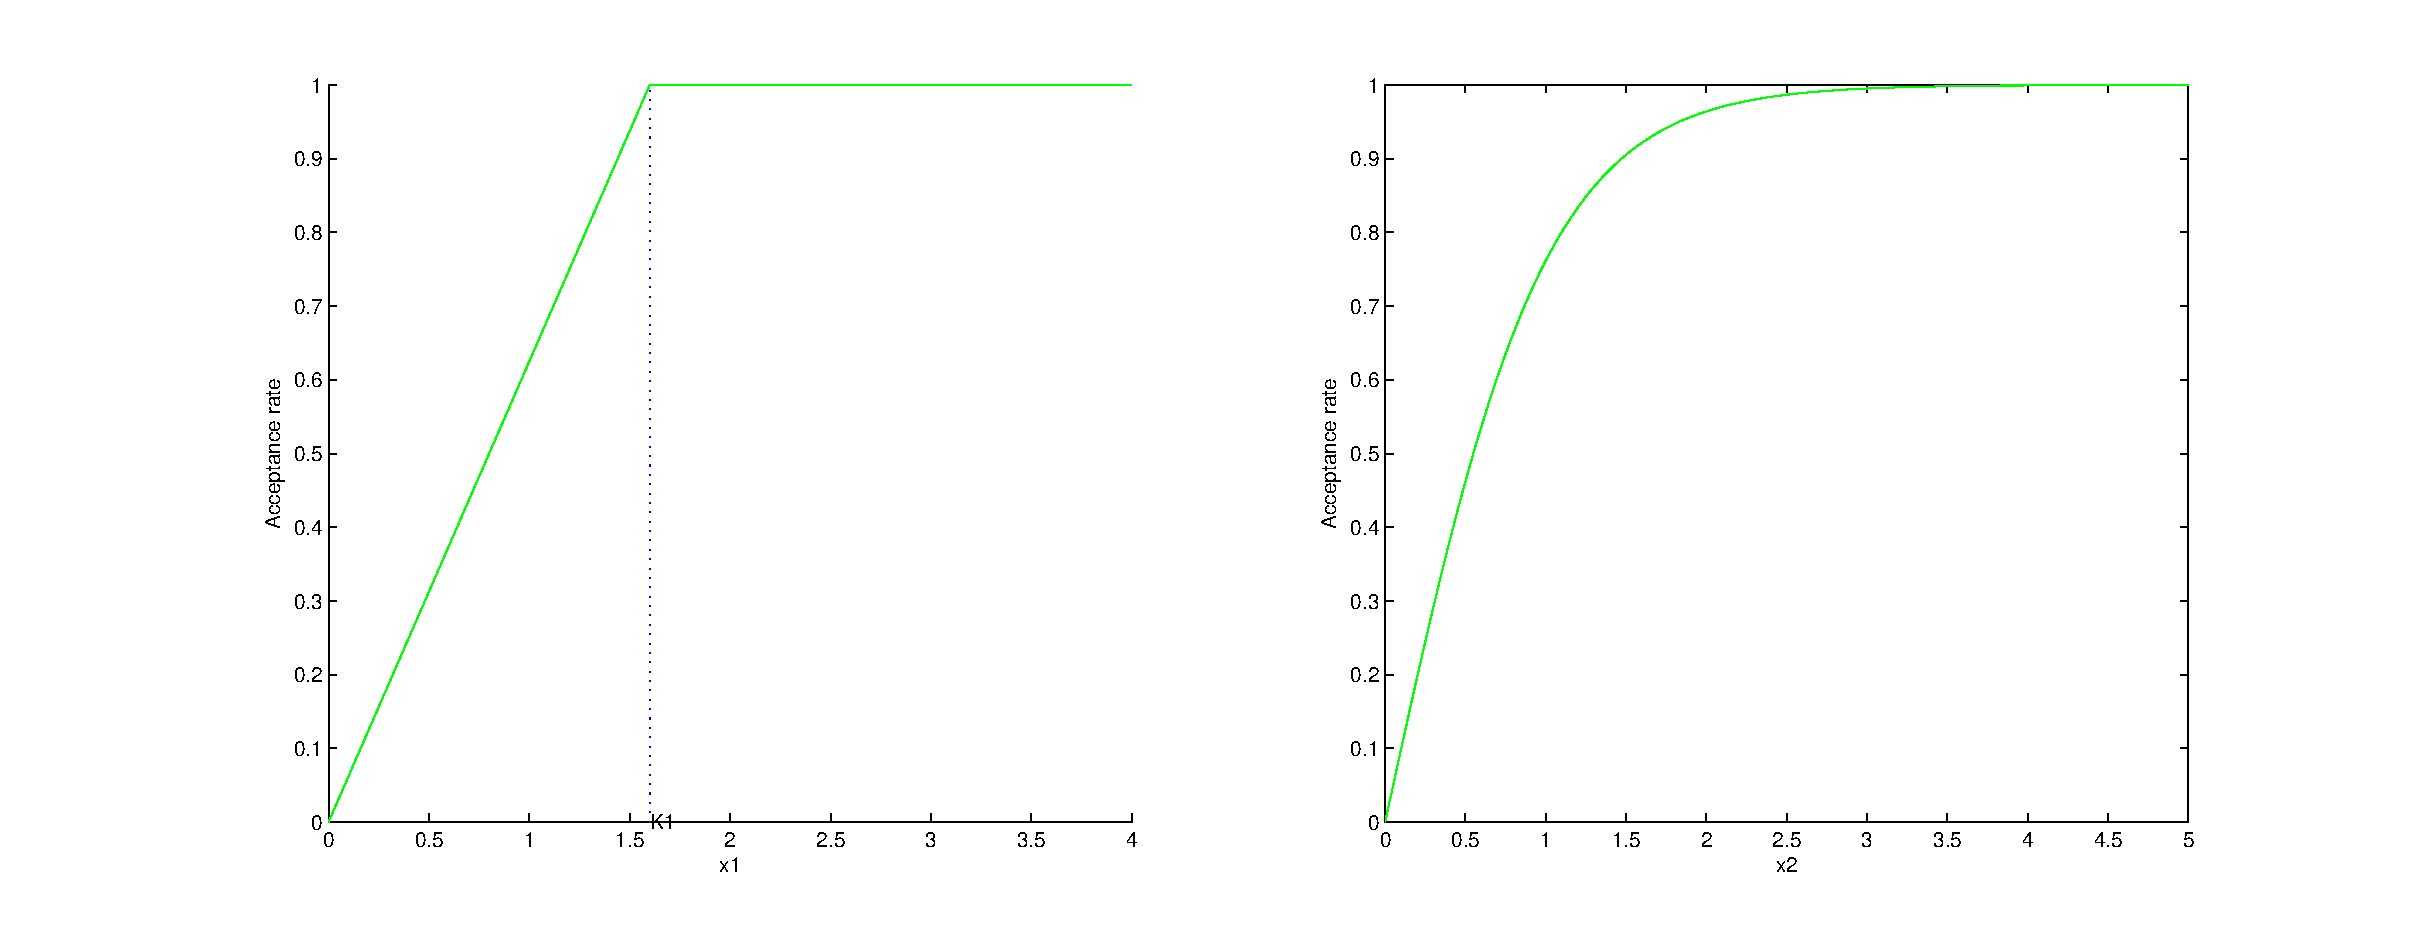
\includegraphics[width=8.5cm]{LinTanh}
\label{img:LinTanh}
\caption{Linear and Hyperbolic Tangent Model}
\end{figure}

\subsubsection{Hyperbolic Tangent Model}
In addition to the above linear model, the hyperbolic tangent function is also considered to model the task acceptance rate.
$$
	AR=\tanh (k_2 \cdot \frac{Rew}{WTD})
$$
Where the $\tanh$ is a hyperbolic tangent function and $k_2$ is the ratio parameter. Let $x_2=k_2 \cdot \frac{Rew}{WTD}$. The hyperbolic tangent function expression is as follows:~\ref{img:TanhModel}
$$
	AR=\tanh (x_2)=\frac{e^{x_2}-e^{-x_2}}{e^{x_2}+e^{-x_2}}
$$

\begin{figure}
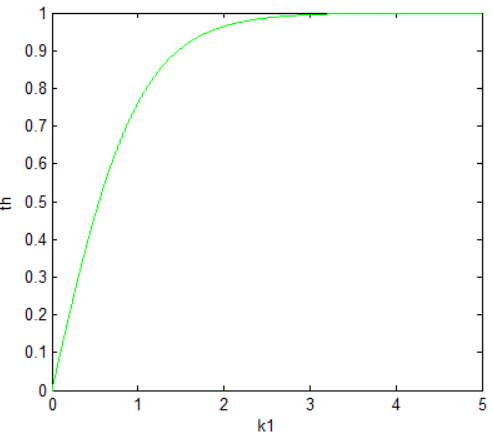
\includegraphics[width=8.5cm]{TanhModel}
\label{img:TanhModel}
\caption{Hyperbolic Tangent Model}
\end{figure}

\subsection{Optimization of Task Acceptance Rate}
We aim to maximize overall $AR$ while satisfying the differential privacy constraints. Considering that the current differential privacy mechanism mainly includes Laplace mechanism and Benders Decomposition linear programming mechanism, we will use these two mechanisms to optimize $AR$.

Unlike Laplace mechanism, the mechanism based on solving linear programming equation with BD algorithm is to transform the location obfuscation function into discrete form $P(L^*|L)$, and the distribution is uncertain in advance, which needs to be iteratively optimized with the task allocation problem (X-subproblem). On the other hand, the obfuscation function of the Laplace mechanism satisfies the planar two-dimensional Laplace distribution, so we only need to adjust the task allocation strategy to optimize $AR$. These are the essential difference between the two ways.

1) Laplace Mechanism

If location $L^* \in \mathbb R^2$ is obtained by adding noise on real location $L_0 \in \mathbb R^2$, the probability density of $L^*$ is negatively exponentially distributed. We aim to maximize the acceptance rate and solve the optimal task allocation strategy. Therefore, we set up linear programming equations is as follows:
$$
	\max \tanh {k \cdot \frac{Rew}{WTD}}
$$
$$
	s.t. \quad P(L^*|L) \propto e^{-\varepsilon d(L^*,L)}
$$
$$
	WTD=\frac {\sum_L \pi(L) P(l^*|L) d(L,L_t)} {\sum_L \pi(L) P(L^*|L)} \chi(L^*,L_t)
$$
$P(L^*|L)$ indicates the probability of obfuscation from location $L$ to $L^*$. $d(L,L_t)$ is the distance between location $L$ and $Lt$. $\pi$ represents the overall location distribution of workers in the location set, ($\sum_L \pi(L)=1$). $\chi(L^*,L_t)$ gives the number of task assignments between workers which located at $L^*$ and tasks which located at $L_t$. 

2) Based on BD algorithm, we set up a linear programming model, and solve optimization goal with differential inequalities and related constraints.
$$
	\max \tanh {k \cdot \frac{Rew}{WTD}}
$$
$$
	s.t. \quad WTD=\frac {\sum_L \pi(L) P(l^*|L) d(L,L_t)} {\sum_L \pi(L) P(L^*|L)} \chi(L^*,L_t)
$$
$$
	P(L^*|L_1) \leq e^{\varepsilon d(L_1,L_2)} P(L^*|L_2) 
$$
$$
	\sum_{L^*} \chi(L^*,L_t)=N_t (L_t)
$$
$$
	\sum_{L^*} P(L^*|L)=1
$$
Unlike the Laplace mechanism, $P(L^*|L)$ here does not follow a specific distribution. It is obtained by solving the linear programming equation iteratively with the task allocation problem (X-subproblem), which satisfies the definition of differential privacy. In the above two equalities, $N_t (L_t)$ represents the total number of tasks located at $L_t$. The total probability that the user’s real location L is obfuscated to other locations is always $1$.

\section{OVERHEAD ANALYSIS}
\subsection{Bandwidth Overhead}
The crowdsourcing server obtains the obfuscation location uploaded by the worker instead of real location. In order to accurately return all tasks within the range $R_w$ of the worker, the crowdsourcing server needs to search with a larger radius near the obfuscation location so that this larger circle with radius $R_{AOR}$ can cover the smaller circle with radius $R_{AOI}$ which is the real range needed to be covered. The larger the search area is, the larger the bandwidth overhead is. (Andrés, Geo-Indistinguishability, CCS’13)

We applied the parameters given by Geo in the calculation of bandwidth overhead - an average of 0.84 KB per POI. Moreover, we assume an average of 20 crowdsourcing tasks per square kilometer. Thus, we can simplify the problem by finding actual search area $S_{AOR}$. Next, the above two obfuscation mechanisms will be analyzed separately.

$S_{AOR}$ can be expressed as a weighted average of multiple areas of search circles. The radius of each search circle is represented by $r_i$, $r_i=d(L^*,L_i)+R_w$. $R_w$ indicates that workers only accept tasks within the range of $R_w$. The diagram is as follows:~\ref{img:AOR}

\begin{figure}
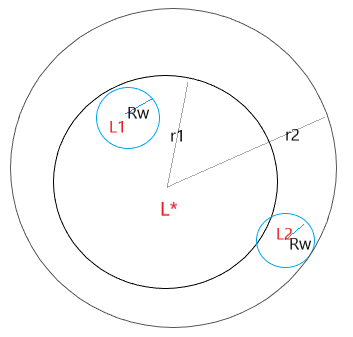
\includegraphics[width=8.5cm]{AOR}
\label{img:AOR}
\caption{Area of Retrieval}
\end{figure}

$$
	S(L^*_k)=\frac{\pi \sum_i P(L^*_k,L_i)(d(L^*_k,L_i)+R_w)^2}{n^2}
$$
$$
	\bar{S}=\frac{\sum_i S(L^*_i)}{N_w}
$$
$P(L^*_k,L_i)$ represents the possibility that location $L_i$ is obfuscated to location $L^*_k$. $S(L^*_k)$ represents the expectation of the actual search area $S_{AOR}$. $N_w$ indicates the number of workers, i.e., number of obfuscated locations uploaded to crowdsourcing server. $\bar{S}$ is the average of $S(L^*_i)$. 

With the mechanism using the Benders Decomposition algorithm, $P(L^*_k,L_i)$ is obtained by solving linear programming problems P and X iteratively. Then we can calculate the corresponding bandwidth overhead from $S_{AOR}$. 

\subsection{Runtime Overhead}
Considering that the locations of workers and crowdsourcing server both need to be continuously updated under practical situations, and the LBS also require real-time performance. Hence it is necessary for us to consider the time overhead.

Since the obfuscation function of the Laplace mechanism is fixed, we only need to adjust the task allocation strategy to optimize the objective function. However, the mechanism based on BD algorithm need to iteratively solve two linear programming problems, i.e., the obfuscation function problem (P-subproblem) and the task allocation problem (X-subproblem), until it converges to the optimization point. As the number of tasks ($N_t$) and the number of workers ($N_w$) increase, the scale of the problem also increases rapidly. As a result, a large number of equalities and inequalities need to be calculated during iteration, which will cause a significant increase of the time overhead.

In the later experiment part, we will observe and compare the time overhead of two mechanisms.

\section{TRADE-OFF BETWEEN PRIVACY AND OVERHEAD}
\subsection{Problem Analysis}
In the differential privacy mechanism, the smaller the privacy budget is, the better the privacy-preserving effect will be. However, since the search area needs to be increased at this time, the search overhead will need to be increased accordingly.

We aim to consider the trade-off between privacy and search overhead comprehensively. First, we use the search area to represent the search overhead. Then, our optimization goal which based on the privacy budget and search area is to reduce the overhead as much as possible while ensuring privacy. Finally, we work out the optimal searching scheme and $\varepsilon$ by minimizing the optimization goal.

\subsection{Trade-off Expression}
We can construct the expression of $S_{AOR}$ as a negative correlation function of $\varepsilon$, i.e., $S(\varepsilon)$, based on the results in section 5.1.2. Then, denote $\hat{\varepsilon}$ as follows:
$$
	\hat{\varepsilon}=\arg \min_\varepsilon \{ \beta \cdot \varepsilon + \ln (S(\varepsilon)) \}
$$
Where $\beta$ is the hyperparameter which can be adjusted according to experience. In this case $\hat{\varepsilon}$ is the optimal point of $\varepsilon$ which not only preserves privacy, but also avoids large expenses.

\section{EXPERIMENT}
Wang(Leye Wang, WWW’17) used the CVX of MATLAB together with the MOSEK in the experiment, as commercial software performs better than open source software. In order to compare two mechanisms, we choose linear programming functions which embedded in MATLAB directly.

\subsection{Optimization Results of Task Acceptance Rate}
In this experiment, we not only compared the Laplace mechanism with the mechanism based on BD algorithm but also considered the no-privacy version, i.e., the locations of workers are uploaded directly to crowdsourcing server without obfuscation. The no-privacy version can be considered as the upper bound of the acceptance rate $AR$. In the experiment, we observed how acceptance rate varied with $N_t$, $N_w$, $\varepsilon$, and $n$. In addition, randomly generated dataset, i.e., the simulated dataset, and the real location dataset, i.e., D4D dataset, are tested and compared respectively. By default, the key parameters are shown in table~\ref{tab:deft}:
\begin{table}
  \caption{Default Value of Key Parameters}
  \label{tab:deft}
  \begin{tabular}{ccl}
    \toprule
    Notation & Default & Description\\
    \midrule
    $N_t$ & $30$ & Number of tasks\\
    $N_w$ & $60$ & Number of workers\\
    $\varepsilon$ & $\ln (4)$ & Privacy budget\\
    $n$ & $4$ & Scale parameter\\
  \bottomrule
\end{tabular}
\end{table}

\subsubsection{Cases with the Linear Model}
The Figure~\ref{img:LinSim} show how acceptance rate varies with $N_t$, $N_w$, $\varepsilon$, and $n$ respectively, using simulated dataset. The threshold $k_1$ of the linear model is set to be $1.6$.

\begin{figure}
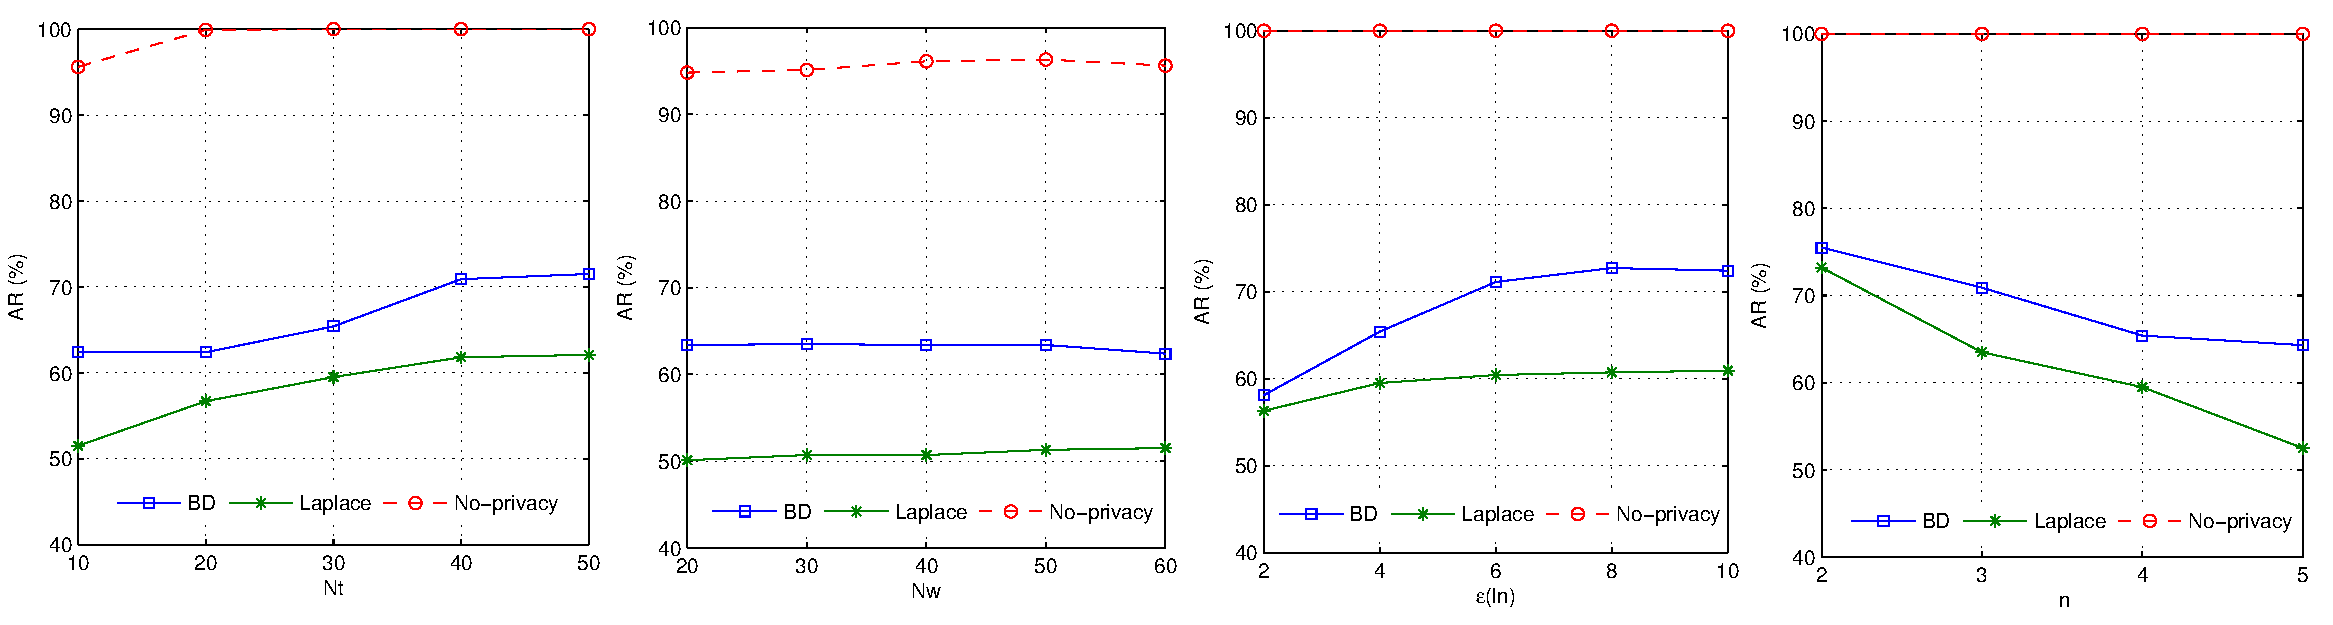
\includegraphics[width=8.5cm]{LinSim}
\label{img:LinSim}
\caption{Linear Model \& Simulated Dataset}
\end{figure}

In addition, we also used the Data for Development (D4D) dataset. This dataset recorded the real locations of the users in communication. The results are shown in Figure~\ref{img:LinD4D}:

\begin{figure}
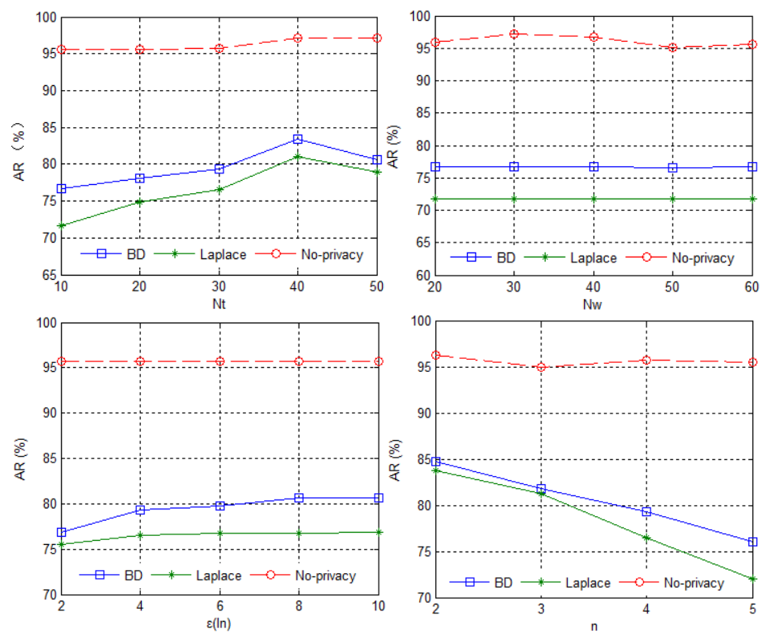
\includegraphics[width=8.5cm]{LinD4D}
\label{img:LinD4D}
\caption{Linear Model \& D4D Dataset}
\end{figure}

By comparing the graphs given by two different datasets, we can conclude that the simulated dataset and the D4D dataset provide approximately the same results. The increase of $N_t$ and $\varepsilon$ can moderately increase the task acceptance rate. The increase of $n$ will reduce the optimization effect of task acceptance rate. Finally, $N_w$ has almost no influence on the result. In this experiment, we assume that $N_t$ is smaller than $N_w$, which means that the increase of $N_t$ has a greater impact on the optimization of task allocation compared with $N_w$. On the other hand, the increase of privacy budget $\varepsilon$ improves the task acceptance rate, which can be seen as sacrificing privacy for performance.

\subsubsection{Cases with Hyperbolic Tangent Model}
We set the ratio parameter $k_2$ in the hyperbolic tangent model to be $0.7$ in the following experiments. Similar to the linear model, we use simulated dataset first, and observe how task acceptance rate varies with $N_t$, $N_w$, $\varepsilon$, and $n$:\ref{img:TanhSim}

\begin{figure}
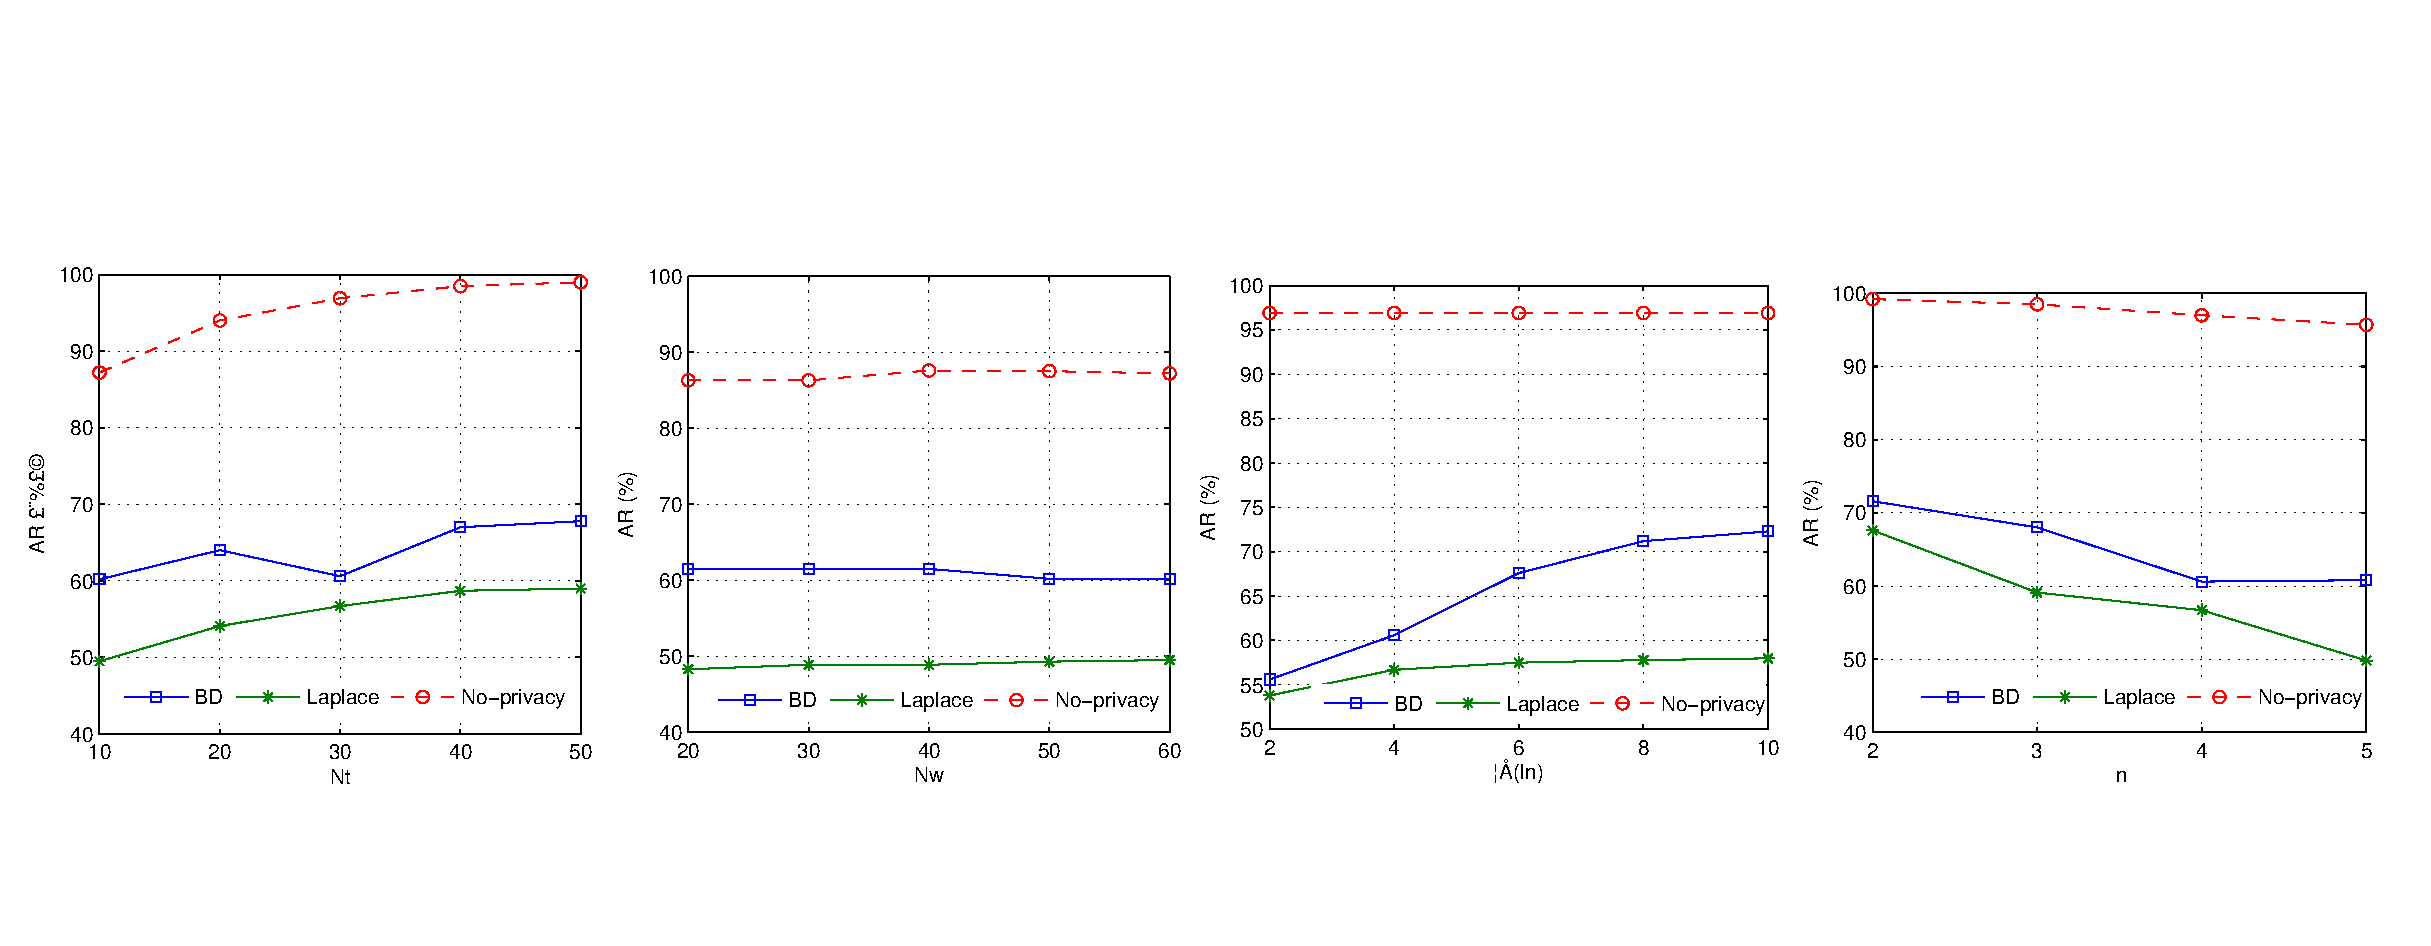
\includegraphics[width=8.5cm]{TanhSim}
\label{img:TanhSim}
\caption{Hyperbolic Tangent Model \& Simulated Dataset}
\end{figure}

Then, results given by D4D dataset follows:\ref{img:TanhD4D}

\begin{figure}
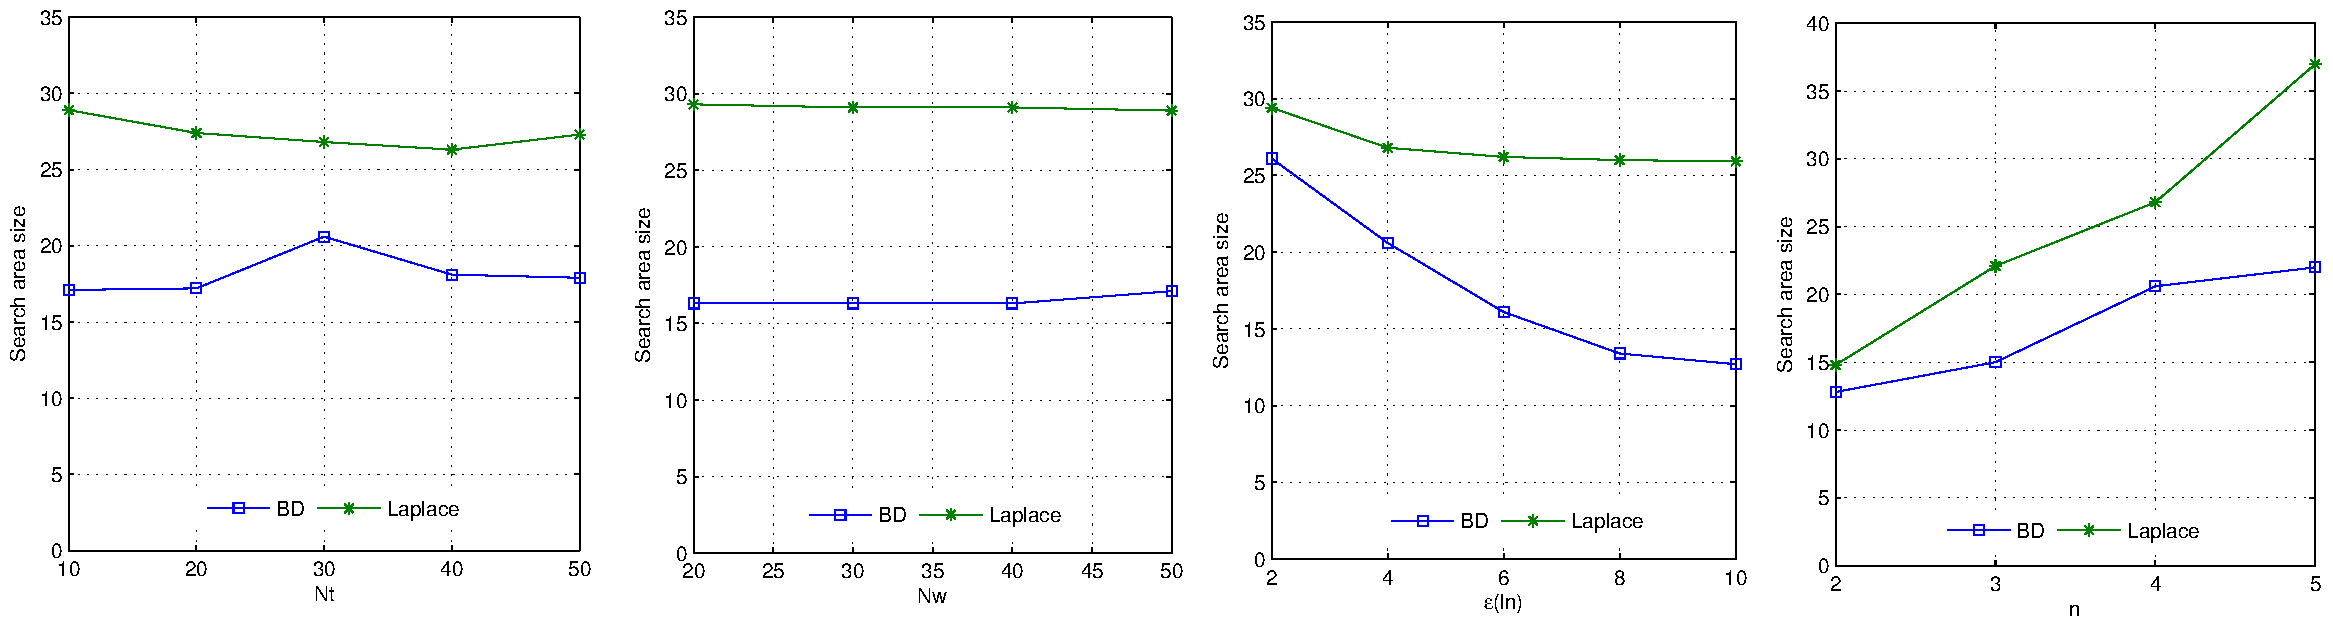
\includegraphics[width=8.5cm]{TanhD4D}
\label{img:TanhD4D}
\caption{Hyperbolic Tangent Model \& D4D Dataset}
\end{figure}

It can be seen that no matter in the linear model or the hyperbolic tangent model, the mechanism based on the BD algorithm outweighs the Laplace mechanism on optimizing the task acceptance rate. Furthermore, increasing $N_t$ and $\varepsilon$ appropriately will improve the task acceptance rate.

\subsection{Overhead Comparison}
\subsubsection{Search Overhead}
In this section, we take the optimization result given by simulated dataset under hyperbolic tangent model as an example and use the search area $S_{AOR}$ to represents the bandwidth overhead. Then, we compare the mechanism based on the BD algorithm and the Laplace mechanism and plot the search area against $N_t$, $N_w$, $\varepsilon$, and $n$ respectively.\ref{img:SAOR}

\begin{figure}
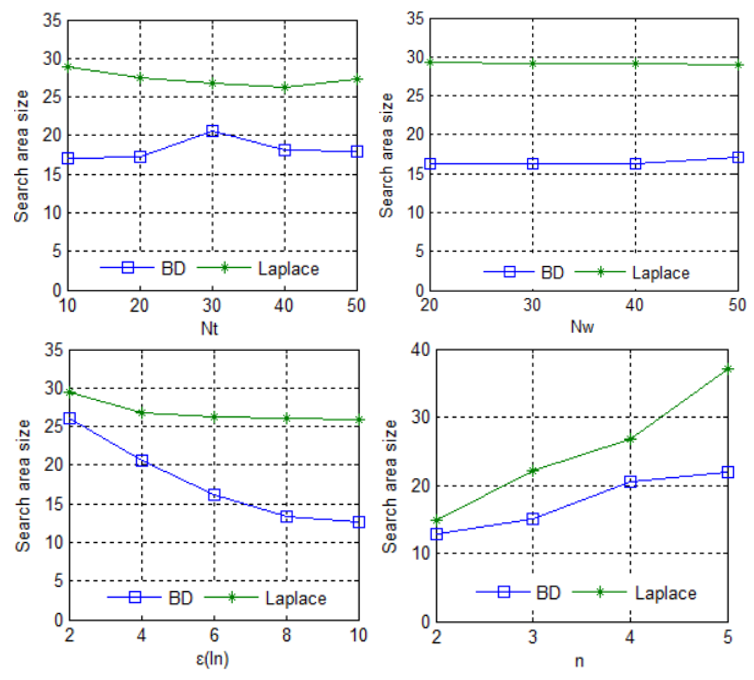
\includegraphics[width=8.5cm]{SAOR}
\label{img:SAOR}
\caption{Search Overhead}
\end{figure}

$\varepsilon$ and $n$ have a significant impact on the search overhead. Reducing privacy and scale parameters can efficiently decrease search overhead. On the other hand, $N_t$ and $N_w$ have little impact.

\subsubsection{Runtime Performance}
Online crowdsourcing has requirements for real-time performance, so it is necessary to consider the runtime overhead. The core idea of BD differential obfuscation mechanism is to decompose the general problem into two subproblems. The optimal solution is obtained by iterating over obfuscation function P and task allocation problem X multiple times, which causes more time overhead.

The environment of the experiment is shown in table~\ref{tab:envi}:
\begin{table}
  \caption{Experiment Platform}
  \label{tab:envi}
  \begin{tabular}{ccl}
    \toprule
    Hardware \& Software & Configuration\\
    \midrule
    Processor & Intel(R)Core(TM)i7-7500U \\
              & CPU@2.70GHz 2.90GHz\\
    Memory & 4GB\\
    Operating System & Windows 10\\
    Operating Environment & MATLAB R2012b\\
  \bottomrule
\end{tabular}
\end{table}

First, considering BD obfuscation mechanism, let $N_w=60$. When $N_t$ varies from $10$ to $50$, the running time is approximately in the range of $35$ to $45$ seconds.

Next, the number of grids $n$ directly determines the number of locations in the location set. Thus, the value of $n$ has a significant impact on the time overhead, which is about $3$ seconds when $n=2$ and about $7$ minutes when $n=5$. The time overhead increases dramatically with the increase of $n$.

Finally, for the Laplace mechanism, let $N_w=60$. When $N_t$ varies from $10$ to $50$, the running time is all within $1$ second. The increase of $n$ has no significant effect on the running time.

\subsection{Curve Fitting and Tradeoff}
We consider the tradeoff between privacy and search overhead according to the trend of search overhead obtained using simulated dataset and the hyperbolic tangent model. First, we construct the expression of $S_{AOR}$ with respect to $\varepsilon$, i.e., $S(\varepsilon)$, that has best fit to the data, and then the optimal privacy budget is selected according to the result of the optimized tradeoff expression.

\subsubsection{Results based on Benders Decomposition}
Based on the BD mechanism, let $N_t=30$, $N_w=60$, we fit the curve to the data points in Figure~\ref{img:CurveBD}.

\begin{figure}
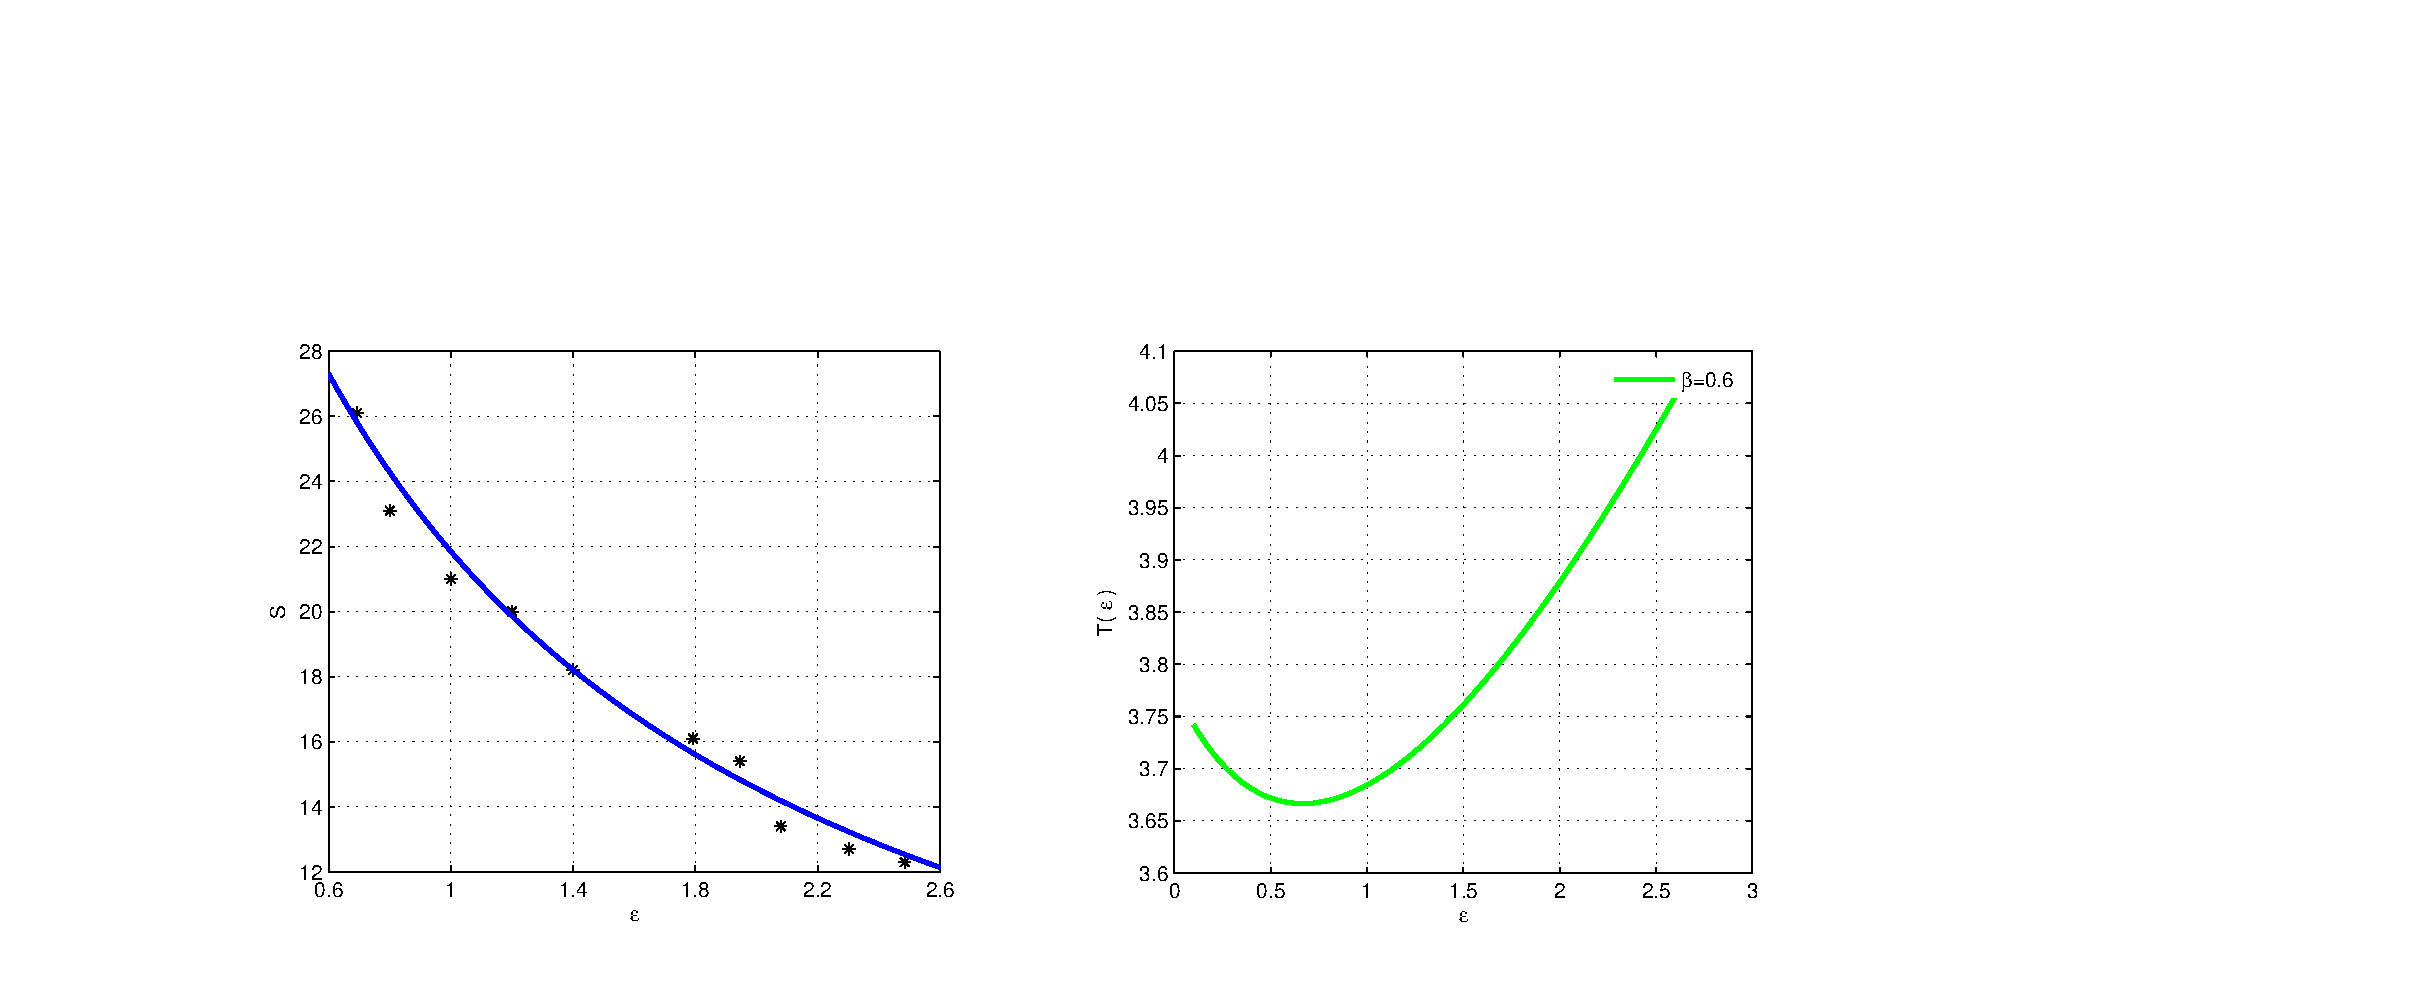
\includegraphics[width=8.5cm]{CurveBD}
\label{img:CurveBD}
\caption{Benders Decomposition Curve Fitting}
\end{figure}

The approximate expression of $S_{AOR}$ is $S(\varepsilon)=\frac{p_1}{\varepsilon + q_1}$, where $p_1=43.7$, $q_1=1.0$. Then we substitute $S(\varepsilon)$ into the tradeoff expression of $\varepsilon$:
$$
	\hat{\varepsilon}=\arg \min_\varepsilon \{ \beta \cdot \varepsilon + \ln (S(\varepsilon)) \} \quad \beta \in (0,1)
$$
When $\beta=0.6$, we plot $\beta \cdot \varepsilon + \ln (S(\varepsilon))$ against $\varepsilon$:\ref{img:TradeoffBD}

\begin{figure}
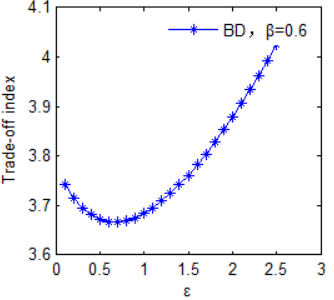
\includegraphics[width=8.5cm]{TradeoffBD}
\label{img:TradeoffBD}
\caption{Tradeoff Expression (BD)}
\end{figure}

The minimum point of the graph corresponds to $\hat{\varepsilon}$, i.e., the optimal $\epsilon$ we seek. At this point, we can think that not only the privacy of the user's location is preserved, but also the excessive search expenses are avoided. 

\subsubsection{Results based on Laplace Mechanism}
Similarly, based on the Laplace mechanism, let $N_t=30$, $N_w=60$, we fit the curve to the data points in Figure~\ref{img:CurveLP}.

\begin{figure}
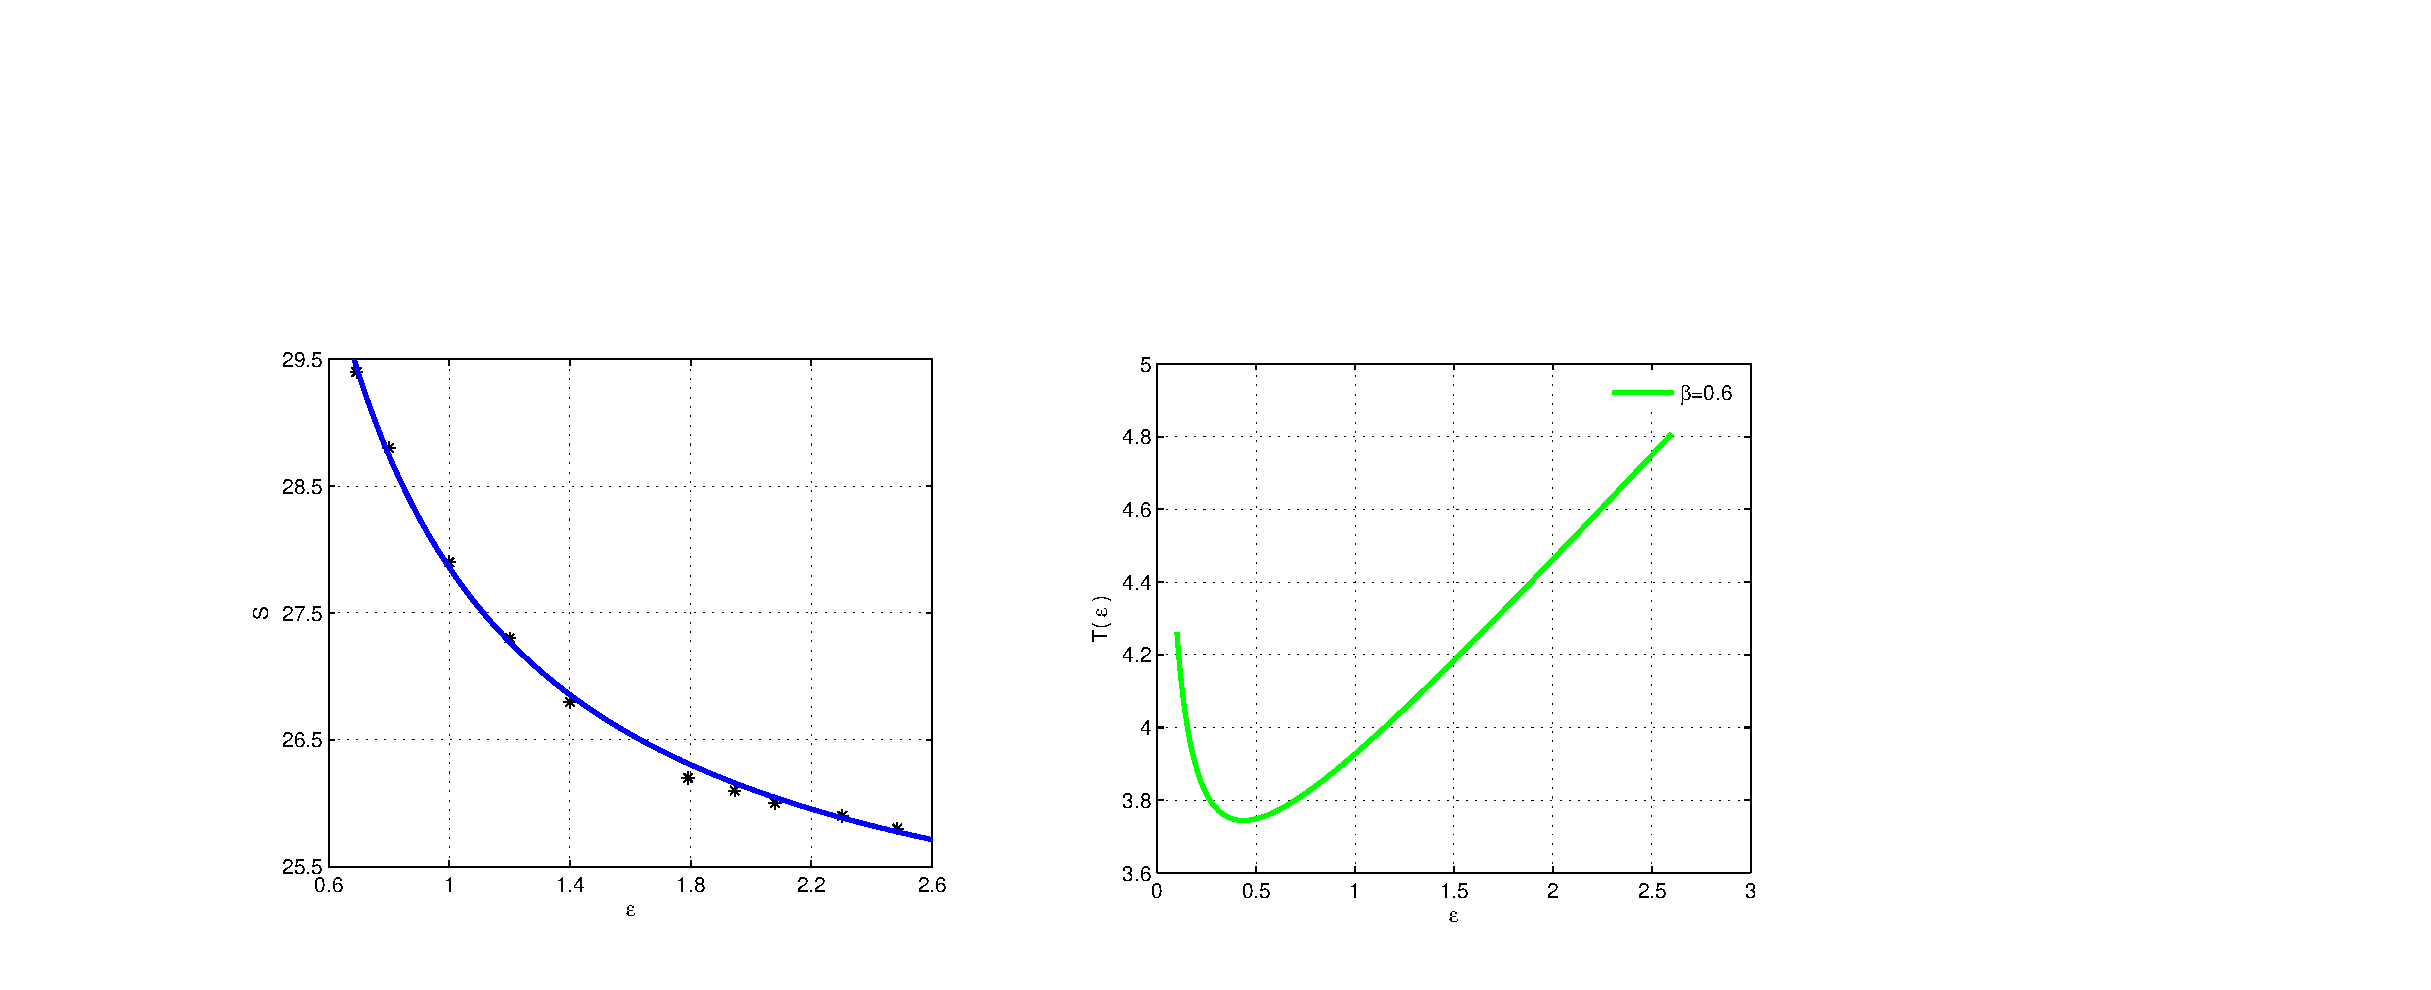
\includegraphics[width=8.5cm]{CurveLP}
\label{img:CurveLP}
\caption{Laplace Curve Fitting}
\end{figure}

The approximate expression of $S_{AOR}$ is $S(\varepsilon)=\frac{p_1 \cdot \varepsilon + p_2}{\varepsilon+q_1}$, where $p_1=24.4$, $p_2=2.9$, $q_1=-0.02$. Then we substitute $S(\varepsilon)$ into the tradeoff expression of $\varepsilon$:
$$
	\hat{\varepsilon}=\arg \min_\varepsilon \{ \beta \cdot \varepsilon + \ln (S(\varepsilon)) \} \quad \beta \in (0,1)
$$
When $\beta=0.6$, we plot $\beta \cdot \varepsilon + \ln (S(\varepsilon))$ against $\varepsilon$:\ref{img:TradeoffLP}

\begin{figure}
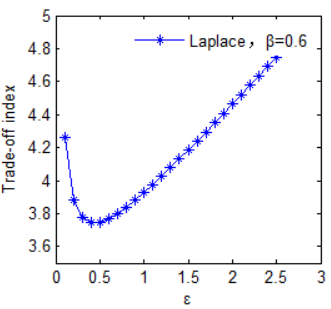
\includegraphics[width=8.5cm]{TradeoffLP}
\label{img:TradeoffLP}
\caption{Tradeoff Expression (LP)}
\end{figure}

The BD mechanism and the Laplace mechanism provide similar results. The minimum point of the graph is the optimal privacy budget that comprehensively weighted privacy and overhead.

\section{CONCLUSION}
In this paper, we improved the model of task acceptance rate under crowdsourcing scenario. We constructed the linear model and the hyperbolic tangent model, and optimized and compared the task acceptance rate with two mainstream mechanisms, i.e., the Laplace mechanism and the mechanism based on solving linear programming with Benders Decomposition algorithm. Generally, the obfuscation function and task allocation strategy based on the BD mechanism can achieve higher task acceptance rate, but it requires more time overhead than the Laplace mechanism and increases significantly with the increase in the size of the problem. In addition, we compared and analyzed the search overhead of two mechanisms. By considering the tradeoff between privacy and search overhead, we gave the best privacy budget choice.
